\documentclass[fontset=windows]{article}
\PassOptionsToPackage{quiet}{fontspec}
\usepackage[a4paper, total={6.5in, 10in}]{geometry}
\usepackage[format=hang,font=small,textfont=it]{caption}
\usepackage{lmodern}
\usepackage{mathtools}
\usepackage{amsmath}
\usepackage{array}
\usepackage{ctex}
\usepackage{cancel}
\usepackage{float}
\usepackage{pifont}
\usepackage{graphicx}
\usepackage{tcolorbox}
\usepackage{tikz}
\usepackage{xcolor}
\usepackage[nottoc]{tocbibind}
\usepackage[hidelinks]{hyperref}
\usepackage{listings}
\definecolor{lightblue}{HTML}{6495ED}
\newcommand*{\mycircled}[1]{\lower
.7ex\hbox{\tikz\draw (0pt, 0pt) circle
(.4em) node {\makebox[0.5em][c]
{\small #1}};}}
\usetikzlibrary{fpu}    % 修理不能使用ifthenelse的错误
\usepackage{pgffor}     % 可以使用foreach的包
\usepackage{ifthen}     % 可以使用ifthenelse的包,还能使用whiledo
\usetikzlibrary{math}   % 使用数学程序

\title{TiKZ技巧}
\author{Eureka}
\date{\today}

\begin{document}
\maketitle
\section{普通环境}
\subsection{支持的运算符}
\begin{itemize}
    \item 1. 判断相等: =
    \item 2. 大于: >
    \item 3. 小于: <
    \item 4. 在普通情况下不能用算数运算符
\end{itemize}

\subsection{基础的foreach循环}
\foreach \x in {1, 2, ..., 20}
{
    \x\hspace*{1em}
}

\subsection{基础的ifthenelse条件语句}
%% 错误的程序: 变量不能够使用/(算术运算符:除法)
% \foreach \i in {1, 2, 3, ..., 10}{
%    \ifthenelse{\i/2 > 5} ... }
\foreach \i in {1, 2, 3, ..., 10}
{
    \ifthenelse{\i < 4}{%
        \i 小于 4;~~~
    }{%
        \i 大于 4;~~~
    }
}

\subsection{基础的ifnum判断}
\newcommand{\Prime}[1]{
    \ifnum #1>4
        #1 > 4
    \fi 
    \ifnum #1=4
        #1 = 4
    \fi 
    \ifnum #1<4
        #1 < 4
    \fi 
}
\Prime{5}
\Prime{4}
\Prime{2}

\section{TiKZMath环境}
tikzmath环境的好处
\begin{itemize}
    \item 1. tikzmath环境内部可以使用算数运算符$+, -, \times, \div$
    \item 2. 还可以使用for循环和if判断
    \item 3. 可以自定义变量和函数
\end{itemize}
\textbf{坏处:只能够在tikzmath环境中,且只能够依赖于tikz输出结果}\par 


\subsection{自定义函数注意事项}
\begin{tikzpicture}
    \tikzmath{%
        function prime(\num, \y){ %
            { \node at (\num, \y) {\num}; };
        };
        % };        %% 错因:函数的调用必须在\tikzmath{}环境内部。不能有空行
        \i = 4;
        %% 测试基本算术运算符
        prime(\i/2, 0);    % 除法
        prime(\i, 0);      % 本身
        prime(\i*2, 0);    % 乘法
        prime(\i+1, 0);    % 加法
        prime(\i-1, 0);    % 减法
        %% 测试内置函数
        prime(sin(\i r), -1);
        prime(exp(\i), -1);
        prime(ln(\i), -1);
        %% 嵌套判断
        function Neg(\num){
            if \num > 0 then{
                {\node at (1, -2) { \num 大于0};};
                % \num 小于0; %% 不能用这种语法,会报错,只能放到node中
            }else{
                % \num 大于0;
               {\node at (3, -2) { \num 小于0};};
            };  %% 注意:else后面有; function后面也有; 函数的调用时使用(),不是{}  
        };
        Neg(-1);
        Neg(1);
    };
\end{tikzpicture}



%% \texorpdfstring{$\alpha$} --> 排除警告:Token not allowed in a PDF string (Unicode):
%%  (hyperref) removing `math shift’.

\subsection{foreach循环与ifthenelse判断}
\begin{figure}[!htb]
    \centering
    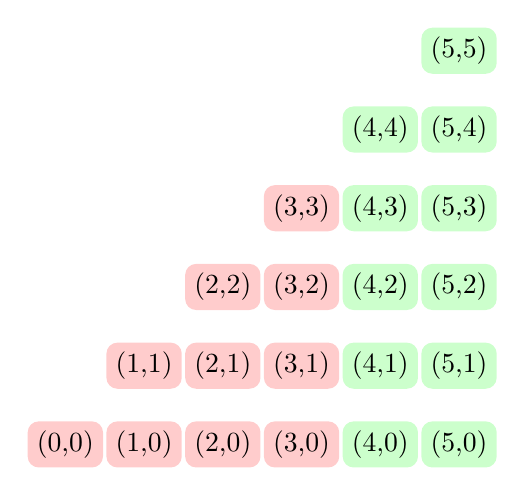
\begin{tikzpicture}
        \foreach \i in {0,...,5}{
            \foreach \j in {0,...,\i}{
                \ifthenelse{\i > 3}{%if成立
                    \node[fill = green!20,rounded corners]at (\i,\j) {(\i,\j)};
                }{%if不成立
                    \node[fill = red!20,rounded corners]at (\i,\j) {(\i,\j)};
                }
            }
        } 
    \end{tikzpicture}
    \caption{foreach循环与ifthenelse判断}
\end{figure}

\subsection{for循环和if判断}
\begin{figure}[!htb]
    \centering
    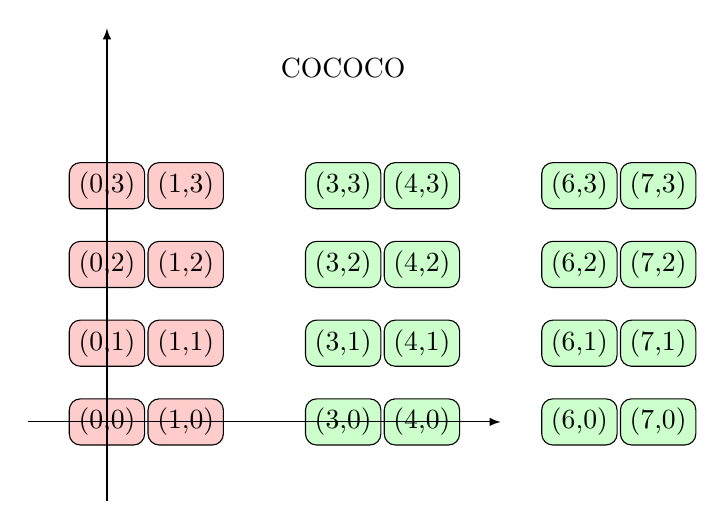
\begin{tikzpicture} 
        \tikzmath{ %数学程序编写,定义的变量可以在其外部使用,里面所有语句都要加分号; 并且不能有多余的回车
            function paint_loop(\x,\y){ %函数中只能使用局部变量,外部变量不能用
                for \i in {0,1,...,\x}{
                    for \j in {0,...,\y}{ 
                        int \ii,\jj; 
                        \ii = \i*1.5; 
                        \jj = \j;  
                        if \ii > 2 then {%条件分支语句    
                            {%绘图代码在数学程序内部使用,要用画括号括起来!!!!
                                \node[draw,fill = green!20,rounded corners] at (\ii,\jj) {(\ii,\jj)};
                            };
                        }else{ 
                            { 
                                \node[draw,fill = red!20,rounded corners] at (\ii,\jj) {(\ii,\jj)};
                            };
                        }; 
                    };
                }; 
            }; 
            \a = 5; %和python一样,加个.就是实数,不加点就是小数
            \b = 3; 
            paint_loop(\a,\b);
            coordinate \co;%能自定义的变量有int、real、coordinate(坐标),不能在定义的时候赋值
            \co = (3,4.5);
        }
        \draw[-latex] (-1,0) -- (5,0);
        \draw[-latex] (0,-1) -- (0,5);
        \node at (\co) {COCOCO}; %在tikzmath中定义的变量在能外部使用
    \end{tikzpicture}
    \caption{for循环和if判断}
\end{figure}



\newpage
\subsection{ifnum判断}
\begin{figure}[!htb]
    \begin{center}
        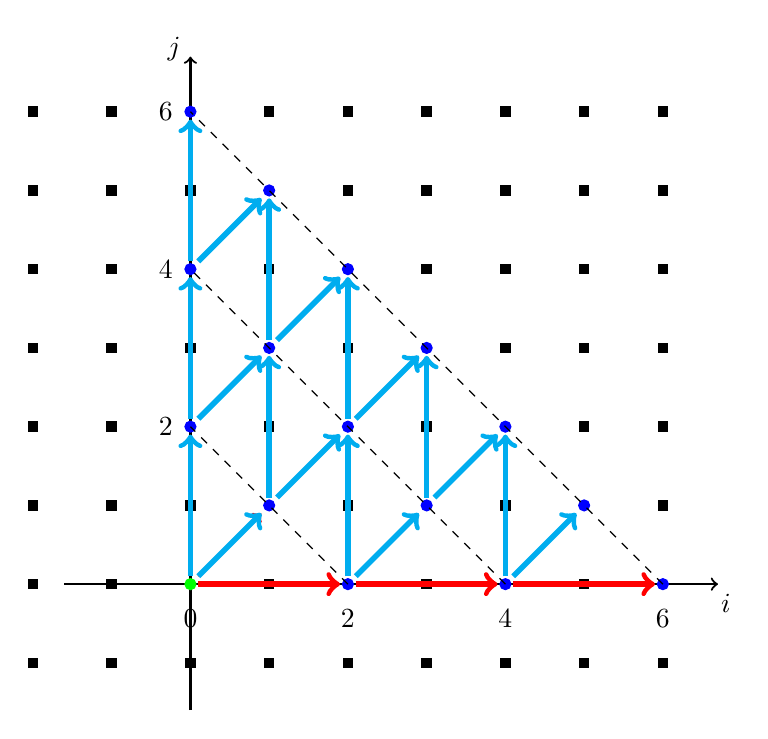
\begin{tikzpicture}
            %% 定义rectangle命令
            \newcommand{\rectangle}[4]{
            \draw[fill, black]
                (#1-0.5*#3, #2-0.5*#4)
                --(#1+0.5*#3, #2-0.5*#4)
                --(#1+0.5*#3, #2+0.5*#4)
                --(#1-0.5*#3, #2+0.5*#4)
                --cycle;
            }
            %% 一些宏定义
            \def\size{0.05}
            \def\boxsize{0.07}
            \def\offset{0.1}
            %% 定义Difirst命令
            \newcommand{\Difirst}[2]{
                \ifnum #1>0
                    \ifnum #2>0
                    \draw[->, line width=2, cyan](#1-1+\offset, #2-1+\offset) to (#1-\offset, #2-\offset);
                    \fi
                \fi
                \ifnum #2>1
                \draw[->, line width=2, cyan](#1, #2-2+\offset) to (#1, #2-\offset);
                \fi
            }
            %% 定义Disecond命令
            \newcommand{\Disecond}[2]{
                \ifnum #1>0
                    \ifnum #2>0
                    \draw[->, line width=2, red](#1-1+\offset, #2-1+\offset) to (#1-\offset, #2-\offset);
                    \fi
                \fi 
                \ifnum #1>1
                \draw[->, line width=2, red](#1-2+\offset, #2) to (#1-\offset, #2);
                \fi 
            }
            %% 定义upright命令
            \newcommand{\upright}[2]{
                \draw[->, thick, red] (#1+0.1, #2+0.1) to (#1+0.9, #2+0.9);
            }
            %% 一系列的绘制命令
            \draw[->, thick] (-1.6, 0)--(6.7, 0);
            \draw[->, thick] (0, -1.6)--(0, 6.7);
            \draw[fill, green] (0, 0) circle [radius=0.07];
            \foreach \t in {0, 2, 4, ..., 6}{
                \ifnum \t>0
                \draw[fill, blue](\t, 0) circle [radius=0.07];
                \fi
                \node[below] at (\t, -0.2) {\t};
            } 
            \foreach \t in {2, 4, ..., 6}{
                \node[left] at (-0.1, \t) {\t};
                \draw[fill, blue] (0, \t) circle [radius=0.07];
            }
            %% 一系列的绘制命令
            \draw[fill, blue] (1, 1) circle [radius=0.07];
            \draw[fill, blue] (1, 3) circle [radius=0.07];
            \draw[fill, blue] (3, 1) circle [radius=0.07];
            \draw[fill, blue] (2, 2) circle [radius=0.07];
            \draw[fill, blue] (1, 5) circle [radius=0.07];
            \draw[fill, blue] (5, 1) circle [radius=0.07];
            \draw[fill, blue] (3, 3) circle [radius=0.07];
            \draw[fill, blue] (2, 4) circle [radius=0.07];
            \draw[fill, blue] (4, 2) circle [radius=0.07];

            %% 绘制小矩形阵列
            % 采用循环绘制小矩形阵列框架
            \foreach \t in {-2, 0, 2, 4, ..., 6}{
                \rectangle{\t}{-1}{0.12}{0.12};
                \rectangle{\t}{1}{0.12}{0.12};
                \rectangle{\t}{3}{0.12}{0.12};
                \rectangle{\t}{5}{0.12}{0.12};
            }
            \foreach \t in {0, 2, 4, ..., 6}{
                \rectangle{\t-1}{0}{0.12}{0.12};
                \rectangle{\t-1}{2}{0.12}{0.12};
                \rectangle{\t-1}{4}{0.12}{0.12};
                \rectangle{\t-1}{6}{0.12}{0.12};
            }

            % 逐句绘制小矩形阵列的中心矩形
            \rectangle{6}{2}{0.12}{0.12};
            \rectangle{6}{4}{0.12}{0.12};
            \rectangle{6}{6}{0.12}{0.12};
            \rectangle{5}{5}{0.12}{0.12};
            \rectangle{5}{3}{0.12}{0.12};
            \rectangle{6}{2}{0.12}{0.12};
            \rectangle{4}{4}{0.12}{0.12};
            \rectangle{4}{6}{0.12}{0.12};
            \rectangle{3}{5}{0.12}{0.12};
            \rectangle{2}{6}{0.12}{0.12};
            \rectangle{5}{-1}{0.12}{0.12}; 
            \rectangle{3}{-1}{0.12}{0.12};
            \rectangle{1}{-1}{0.12}{0.12};
            \rectangle{-1}{-1}{0.12}{0.12};
            \rectangle{-1}{1}{0.12}{0.12};
            \rectangle{-1}{3}{0.12}{0.12};
            \rectangle{-1}{5}{0.12}{0.12};
            \rectangle{-2}{0}{0.12}{0.12};
            \rectangle{-2}{2}{0.12}{0.12};
            \rectangle{-2}{4}{0.12}{0.12};
            \rectangle{-2}{6}{0.12}{0.12};
            \draw[dashed] (2, 0)--(0, 2);
            \draw[dashed] (4, 0)--(0, 4);
            \draw[dashed] (6, 0)--(0, 6);
            \upright{0}{0};

            %% 绘制Dfirst
            \Difirst{0}{2};
            \Difirst{0}{4};
            \Difirst{0}{6};
            \Difirst{1}{1};
            \Difirst{2}{2};
            \Difirst{1}{3};
            \Difirst{3}{1};
            \Difirst{1}{5};
            \Difirst{2}{4};
            \Difirst{3}{3};
            \Difirst{4}{2};
            \Difirst{5}{1};
            \Disecond{2}{0};
            \Disecond{4}{0};
            \Disecond{6}{0};
            \node[below] at (6.8, 0) {$i$};
            \node[left] at (0, 6.8) {$j$};
        \end{tikzpicture} 
        \caption{Algorithm of the triangle integral with $m=6$}
        \label{Tri-Figure}
    \end{center}
\end{figure}

\subsection{综合:绘制神经网络}
\begin{figure}[!htb]
    \centering
    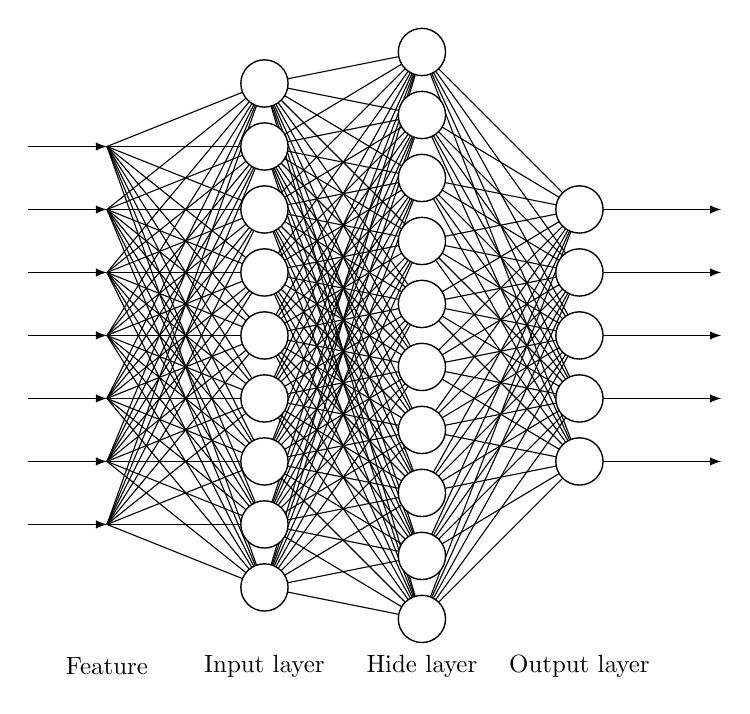
\begin{tikzpicture} 
        \tikzmath{ 
            function paint_nodes(\radius,\gapy,\posx,\num){ 
                \gapy = \gapy+\radius*2;  
                \starty = \gapy*(\num-1)/2; 
                for \i in {0,...,\num-1}{
                    \drawy = \starty - \i*\gapy; 
                    {
                        \filldraw[line width = 0.5pt,fill = white] (\posx,\drawy) circle (\radius);
                    };
                };   
            };
            function paint_lines(\radius,\gapy,\posx,\num,\nextposx,\nextnum){ 
                \gapy = \gapy+\radius*2;  
                \starty = \gapy*(\num-1)/2;
                \startyy = \gapy*(\nextnum-1)/2; 
                for \i in {0,...,\num-1}{
                    \drawy = \starty - \i*\gapy; 
                    for \j in {0,...,\nextnum-1}{  
                        \drawyy = \startyy - \j*\gapy;   
                        {
                            \draw (\posx,\drawy) -- (\nextposx,\drawyy);
                        };
                    }; 
                };
            };
            function paint_x_lines(\radius,\gapy,\posx,\num,\ifright,\len){
                \gapy = \gapy+\radius*2;  
                \starty = \gapy*(\num-1)/2; 
                for \i in {0,...,\num-1}{
                    \drawy = \starty - \i*\gapy; 
                    if \ifright == 1 then{
                        {
                            \draw[-latex] (\posx,\drawy) -- (\posx+\len,\drawy);
                        }; 
                    }else{ 
                        {
                            \draw[-latex] (\posx,\drawy)--(\posx-\len,\drawy);
                        }; 
                    }; 
                }; 
            };
            function paint_net(\x0,\x1,\x2,\x3){  
                \gapx = 2;
                \radius = 0.3;
                \gapy = 0.2; 
                paint_lines(\radius,\gapy,0*\gapx,\x0,1*\gapx,\x1);
                paint_lines(\radius,\gapy,1*\gapx,\x1,2*\gapx,\x2);
                paint_lines(\radius,\gapy,2*\gapx,\x2,3*\gapx,\x3); 
                paint_x_lines(\radius,\gapy,3*\gapx,\x3,1,1.8);
                paint_x_lines(\radius,\gapy,0*\gapx-1,\x0,1,1);
                paint_nodes(\radius,\gapy,1*\gapx,\x1); 
                paint_nodes(\radius,\gapy,2*\gapx,\x2);
                paint_nodes(\radius,\gapy,3*\gapx,\x3);  
            };  
            paint_net(7,9,10,5); 
        } 
        \node[scale = 0.9] at (0,-4.2) {Feature};
        \node[scale = 0.9] at (2,-4.2) {Input layer};
        \node[scale = 0.9] at (4,-4.2) {Hide layer};
        \node[scale = 0.9] at (6,-4.2) {Output layer}; 
    \end{tikzpicture}    
    \caption{绘制神经网络}
\end{figure}

\end{document}

